%%
%% Heterogeneous Adapters for AI-Agent Observability:
%% A Middleware Architecture for Span Correlation Across
%% Callback, Hook, and Monkey-Patch Instrumentation
%%
%% Target: ACM/IFIP Middleware 2026 Cycle 2 (12 pp + refs, ACM SIGCONF 9pt, double-blind)
%%

\documentclass[sigconf,review,anonymous,9pt]{acmart}

%% ---------- packages ----------
\PassOptionsToPackage{hyphens}{url}
\usepackage{booktabs}
\usepackage{enumitem}
\usepackage{multirow}
\let\Bbbk\relax
\usepackage{amssymb}
\usepackage{microtype}
\usepackage{balance}
\usepackage{tikz}
\usepackage{listings}
\usepackage{xcolor}
\usetikzlibrary{positioning,arrows.meta,shapes.geometric,fit,backgrounds,calc}

%% Allow LaTeX to stretch lines when needed to avoid right-margin overflow
\setlength{\emergencystretch}{3em}
\tolerance=2000
\hfuzz=2pt
\hbadness=10000

%% URL break sensitivity
\makeatletter
\g@addto@macro\UrlBreaks{\do\_\do\.\do\-\do\,\do\?\do\/}
\makeatother

%% Listings style for code snippets
\lstdefinestyle{pyminimal}{%
  basicstyle=\ttfamily\fontsize{7.5}{8.8}\selectfont,
  keywordstyle=\bfseries,
  commentstyle=\itshape\color{black!55},
  showstringspaces=false,
  numbers=none,
  frame=single,
  rulecolor=\color{black!50},
  framesep=2pt,
  columns=fullflexible,
  keepspaces=true,
  language=Python,
  breaklines=true,
  upquote=true,
}

%% ---------- conference metadata (double-blind, generic placeholders) ----------
%% printacmref=false: ACM reference block requires DOI/year/venue that would
%% de-anonymize the submission. The mandatory ACM reference format is
%% supplied with the camera-ready version per CFP.
%% printccs=true: CCS concepts are CFP-mandatory for papers over 2 pages.
\settopmatter{printacmref=false,printccs=true,printfolios=true}
\setcopyright{none}
\acmConference[Middleware '26]{27th ACM/IFIP International Middleware Conference}{14--18 December 2026}{Tarragona, Spain}
\acmYear{2026}
\copyrightyear{2026}
\acmISBN{}
\acmDOI{}

\renewcommand\footnotetextcopyrightpermission[1]{}

%% ---------- title and (anonymized) author block ----------
\title[Heterogeneous Adapters for AI-Agent Observability]{Heterogeneous Adapters for AI-Agent Observability:\\A Middleware Architecture for Span Correlation\\Across Callback, Hook, and Monkey-Patch Instrumentation\\\normalsize{[Research]}}

\author{Anonymous Author(s)}
\affiliation{%
  \institution{Submission \#XXX}
  \city{}
  \country{}
}
\email{anon@anon.invalid}

%% ---------- begin document ----------
\begin{document}

\begin{abstract}
\sloppy
AI-agent systems built on heterogeneous frameworks---LangChain, CrewAI,
AutoGen, LlamaIndex, and direct LLM SDKs---resist a unified
observability layer because each framework exposes a structurally
different extensibility surface. LangChain ships a callback registry;
CrewAI exposes a typed hook system; the OpenAI, Anthropic, and AutoGen
SDKs offer none and must be monkey-patched. We present a middleware
architecture that reconciles these three incompatible instrumentation
paradigms under a single semantic-convention overlay built on
OpenTelemetry. The architecture has three tiers: a semantic substrate
that encodes nine agent-specific span kinds as attributes on
OpenTelemetry \texttt{INTERNAL} spans (working around OTel's fixed
five-value \texttt{SpanKind} enum); a set of seven lazy-imported
adapters, one per framework, each implementing the OpenTelemetry
\texttt{BaseInstrumentor} contract via the strategy native to its host;
and a pluggable analysis pipeline that consumes the exported span
stream for anomaly detection, cost aggregation, decision attribution,
and hallucination tracing. Cross-agent trace context is propagated by
extending W3C trace-context baggage with agent-identity fields,
permitting correlation across synchronous in-process delegation,
asyncio task boundaries, and multi-process agent topologies. We
evaluate the architecture on six framework adapters across six
telemetry conditions on a 3{,}780-cell measurement matrix. Per-span
overhead is 11--13~\textmu s at p50 and 27--43~\textmu s at p99 across
the nine span kinds; the middleware sustains 78{,}087 spans/s
in-memory and 19{,}071 spans/s under 100-thread concurrency.
End-to-end agent overhead at the SDK's default privacy level ranges
from $+$0.41~ms (Anthropic monkey-patch) to $+$1.83~ms (CrewAI hook),
mean $+$1.07~ms. On a paired per-adapter basis the default
configuration adds $+$0.92~ms versus $+$2.12~ms for vanilla
OpenTelemetry, $+$2.16~ms for OTel GenAI, and $+$2.20~ms for
OpenInference, averaged across the five non-CrewAI adapters; the
per-adapter 95\% paired-delta confidence intervals are non-overlapping
on four of those five adapters (LangChain, LlamaIndex, OpenAI,
Anthropic), making the lower overhead statistically significant
rather than a single-run artifact. The middleware delivers
nine-of-nine span-kind coverage versus two-of-nine for vanilla
OpenTelemetry, OTel GenAI, and OpenInference. The architecture is
implemented in 3{,}762 lines of Python over 78 tests, and its source
materials are available to reviewers via an anonymized submission
archive.
\end{abstract}

%% ---------- CCS concepts (ACM-mandatory for >2p) ----------
\begin{CCSXML}
<ccs2012>
   <concept>
       <concept_id>10011007.10011074.10011099.10011102.10011103</concept_id>
       <concept_desc>Software and its engineering~Software performance</concept_desc>
       <concept_significance>500</concept_significance>
       </concept>
   <concept>
       <concept_id>10011007.10010940.10011003.10011002</concept_id>
       <concept_desc>Software and its engineering~Software reliability</concept_desc>
       <concept_significance>300</concept_significance>
       </concept>
   <concept>
       <concept_id>10010520.10010575.10010755</concept_id>
       <concept_desc>Computer systems organization~Reliability</concept_desc>
       <concept_significance>300</concept_significance>
       </concept>
   <concept>
       <concept_id>10011007.10011074.10011092.10011093</concept_id>
       <concept_desc>Software and its engineering~Software libraries and repositories</concept_desc>
       <concept_significance>300</concept_significance>
       </concept>
   <concept>
       <concept_id>10010147.10010178.10010187.10010195</concept_id>
       <concept_desc>Computing methodologies~Multi-agent systems</concept_desc>
       <concept_significance>300</concept_significance>
       </concept>
 </ccs2012>
\end{CCSXML}

\ccsdesc[500]{Software and its engineering~Software performance}
\ccsdesc[300]{Software and its engineering~Software reliability}
\ccsdesc[300]{Computer systems organization~Reliability}
\ccsdesc[300]{Software and its engineering~Software libraries and repositories}
\ccsdesc[300]{Computing methodologies~Multi-agent systems}

%% ---------- keywords (ACM-mandatory for >2p) ----------
\keywords{AI agents, observability, OpenTelemetry, distributed tracing, middleware, instrumentation, span correlation, large language models}

\maketitle

%% =====================================================================
\section{Introduction}
%% =====================================================================

Autonomous AI-agent systems---LLM-driven processes that plan,
delegate, invoke tools, and consult external knowledge sources---are
increasingly deployed in production
settings~\cite{mast,aegis,agentdebug}. Unlike the single-process
microservices that distributed-tracing middleware was designed
for~\cite{dapper,jaeger,zipkin}, contemporary agent deployments
typically combine \emph{multiple} frameworks within a single
application: a LangChain~\cite{langchain} orchestration layer might
delegate to a CrewAI~\cite{crewai} multi-agent crew that calls the
OpenAI SDK~\cite{openai_sdk} for one LLM and the Anthropic
SDK~\cite{anthropic_sdk} for another, while LlamaIndex~\cite{llamaindex}
handles retrieval and AutoGen~\cite{autogen} mediates inter-agent
conversation. An operator who wants a single coherent trace across
this stack faces a fragmentation problem that is structural, not
incidental.

The structural problem is that each framework exposes a different
\emph{instrumentation surface}. LangChain and LlamaIndex offer
first-class callback (respectively, hook) APIs that can be cleanly
subscribed at startup. CrewAI exposes a typed hook system distinct
from LangChain's. The OpenAI, Anthropic, and AutoGen SDKs expose no
public extensibility surface for tracing, requiring instrumentation
that wraps imported classes at load time. Existing LLM-observability
products~\cite{langsmith,langfuse,openllmetry,openinference} either
target a single framework, or bundle a fixed set of adapters that all
follow one strategy, or rely on the user to manually emit spans.
There is no published middleware architecture that reconciles
\emph{three} structurally different instrumentation paradigms under a
common semantic layer, with quantified per-adapter overhead, and with
a context-propagation story validated across asynchronous multi-agent
topologies. This paper presents such an architecture.

\textbf{What is new in two sentences.} Prior agent-observability
work either targets one framework with one strategy (e.g.,
LangSmith's LangChain-only callback path) or layers a vocabulary on
top of OpenTelemetry without addressing the heterogeneous
instrumentation surface (OTel GenAI conventions, OpenInference);
no prior system reconciles callback, hook, and monkey-patch
strategies under a single agent-semantic overlay with a
quantified-overhead and validated-context-propagation story. We
present the first such reconciliation, codify it as three explicit
middleware contracts, and show on a paired-delta benchmark that the
resulting overhead is statistically significantly lower than every
named baseline on four of five non-CrewAI adapters.

\textbf{Why this is harder than it looks.} Each of the three
instrumentation strategies has its own failure mode: callbacks must
preserve handler ordering and exception propagation; hooks must
demultiplex across overlapping pre-/post- event types; monkey-patches
must be idempotent, restorable, and survive minor-version drift in
the patched class. Composing the three under a single user-facing API
forced redesigns of the lazy-import sequence (an early implementation
deadlocked under specific framework loading orders), the
\texttt{BaseInstrumentor} contract surface (so that an OTel deployment
already using the contrib pattern composes without conflict), and the
baggage-carrier format (which must round-trip across in-process,
asyncio, and multi-process boundaries without losing the
agent-identity fields). The architecture in \S\ref{sec:arch} is the
fourth iteration; the first three crashed in production-shape stress
tests.

Our framing is deliberately a \emph{middleware} contribution. Recent
agent-observability work focuses on the semantics of fault
detection~\cite{aegis,agentdebug,agentrx}, the taxonomy of agent
failures~\cite{mast}, or post-hoc tracing
analyses~\cite{agdebugger,agentops}. These are valuable but they
treat the underlying instrumentation layer as a solved problem. It is
not. The instrumentation layer is where the heterogeneity bites; it
is where overhead is paid; it is where trace correlation either
succeeds or silently fails. A middleware-research treatment of this
layer is overdue. The classical RPC-tracing literature
(Dapper~\cite{dapper}, Pinpoint~\cite{pinpoint},
X-Trace~\cite{xtrace}, Magpie~\cite{magpie}) assumed a homogeneous
extensibility surface---a single servlet filter or gRPC interceptor
chain---and so did not need to reconcile structurally different
adapter strategies. Agent middleware does.

\textbf{Contributions.}
\begin{itemize}[leftmargin=*,nosep]
  \item A three-tier middleware architecture that reconciles
    callback-based, hook-based, and monkey-patch instrumentation under
    a single agent-aware semantic-convention overlay on OpenTelemetry,
    with explicit design principles (lazy-import discipline,
    attribute-overlay encoding, decoupled analysis pipeline) elevated
    from engineering practice to stated middleware contracts
    (\S\ref{sec:arch}).
  \item A W3C-baggage extension that propagates agent identity
    across synchronous in-process delegation, asyncio task
    boundaries, and multi-process delegation, with a carrier
    format and an idempotency argument (\S\ref{sec:arch}).
  \item An empirical evaluation across six framework adapters and six
    telemetry conditions (3{,}780 measured cells from a
    fault-injection matrix) reporting per-span overhead at p50/p95/p99,
    end-to-end agent run-time per adapter with paired 95\%
    confidence intervals, span-kind coverage relative
    to vanilla OpenTelemetry, OpenTelemetry GenAI semantic
    conventions, and OpenInference~\cite{openinference}, and
    multi-agent topology correlation across hierarchical, parallel,
    and sequential configurations (\S\ref{sec:eval}).
  \item A scalability stress test demonstrating 78{,}087 spans/s
    in-memory and 19{,}071 spans/s under 100-thread concurrency, with
    backpressure characterisation under disk-backed export
    (\S\ref{sec:eval}).
\end{itemize}

The middleware is implemented in 3{,}762 lines of Python distributed
over 78 unit and integration tests; the source materials are available
to reviewers via the anonymized submission archive and re-running the
evaluation requires a single shell command documented in
\S\ref{sec:impl}.

%% =====================================================================
\section{Background and Motivation}
\label{sec:bg}
%% =====================================================================

\subsection{OpenTelemetry SDK architecture}

OpenTelemetry~\cite{otel} (OTel) is the de facto open standard for
distributed tracing. Its SDK is structured as a pipeline: a
\texttt{TracerProvider} owns a \texttt{Sampler}, one or more
\texttt{SpanProcessor}s, and one or more \texttt{Exporter}s. Spans
emitted by application code (typed by a five-value \texttt{SpanKind}
enum: \texttt{INTERNAL}, \texttt{CLIENT}, \texttt{SERVER},
\texttt{PRODUCER}, \texttt{CONSUMER}) flow through processors that
batch, sample, or attribute them, then to exporters that ship them to
a backend (Jaeger~\cite{jaeger}, Tempo~\cite{tempo}, or a vendor
APM~\cite{datadog_apm}). The \emph{semantic convention} layer above
the SDK standardises attribute names so that, e.g., an HTTP server
span looks the same regardless of which language SDK emitted it.

The agent-observability problem inherits OTel's pipeline architecture
but exposes a gap in the semantic layer: OTel's \texttt{SpanKind}
enum is closed, and the OTel GenAI semantic
convention~\cite{otel_genai_semconv} (the most recent specification at
the time of writing) defines attribute names only for LLM invocation
and tool execution. It does not name the orchestration phases that
agent systems care about---planning, reasoning, safety monitoring,
inter-agent delegation, and memory access. Our middleware therefore
needs to add a vocabulary, not just an adapter set.

\subsection{The AI-agent framework landscape}

We surveyed six widely used agent frameworks (Table~\ref{tab:adapters})
plus a manual API for custom agents. The frameworks fall into three
distinct extensibility categories:

\textbf{Callback-based.} LangChain~\cite{langchain} exposes a
callback registry where user code subclasses
\texttt{BaseCallbackHandler} and registers an instance with the
runtime. Lifecycle events (\texttt{on\_chain\_start},
\texttt{on\_tool\_end}, etc.) are then dispatched to the handler in
deterministic order. The middleware adapter dynamically constructs a
callback subclass at instrument time, avoiding an import-time
dependency on the host framework.

\textbf{Hook-based.} CrewAI~\cite{crewai} ships a typed hook system:
pre-/post- hooks for task execution and for LLM invocation are
registered through a domain-specific API. LlamaIndex's modern
\texttt{instrumentation} module~\cite{llamaindex} similarly exposes a
\texttt{BaseSpanHandler} subclass point. This is structurally a
different surface from callbacks: the registration API is typed and
the event semantics differ. Although it falls into the broad
``first-class extensibility'' category alongside callbacks, the
adapter implementation is not interchangeable with a callback-based
one.

\textbf{Monkey-patch.} The OpenAI Python SDK~\cite{openai_sdk}, the
Anthropic Python SDK~\cite{anthropic_sdk}, and AutoGen~\cite{autogen}
expose no public extensibility surface for tracing. The adapter must
replace methods on
\texttt{openai.resources.chat.completions.Completions},
\texttt{anthropic.resources.messages.Messages}, and
AutoGen's core agent classes at instrument time. The patched method
invokes the original and wraps the call in a span. This strategy is
brittle (a version bump can rename a method) and demands a lazy-import
discipline (a single SDK installation must not pull in all three
vendor packages).

The challenge for a middleware is to expose one user-facing API
(\texttt{configure(...)} plus \texttt{Instrumentor.instrument()})
over three structurally incompatible adapter strategies, while
keeping overhead low, dependencies optional, and trace context
propagated across heterogeneous boundaries. Adjacent literature
exists in the Java APM tradition, embodied by the OpenTelemetry Java
agent~\cite{otel_java_agent} and predecessors such as
Pinpoint~\cite{pinpoint}. That tradition has long maintained
heterogeneous instrumentation through bytecode rewriting, a
mechanism that collapses to one strategy (bytecode AOP) regardless
of target. Our setting differs because Python has no equivalent
bytecode-rewriting culture; the strategy mix is the natural shape of
the problem, not an implementation accident.

%% =====================================================================
\section{Middleware Architecture}
\label{sec:arch}
%% =====================================================================

\begin{figure*}[t]
\centering
\resizebox{0.92\textwidth}{!}{%
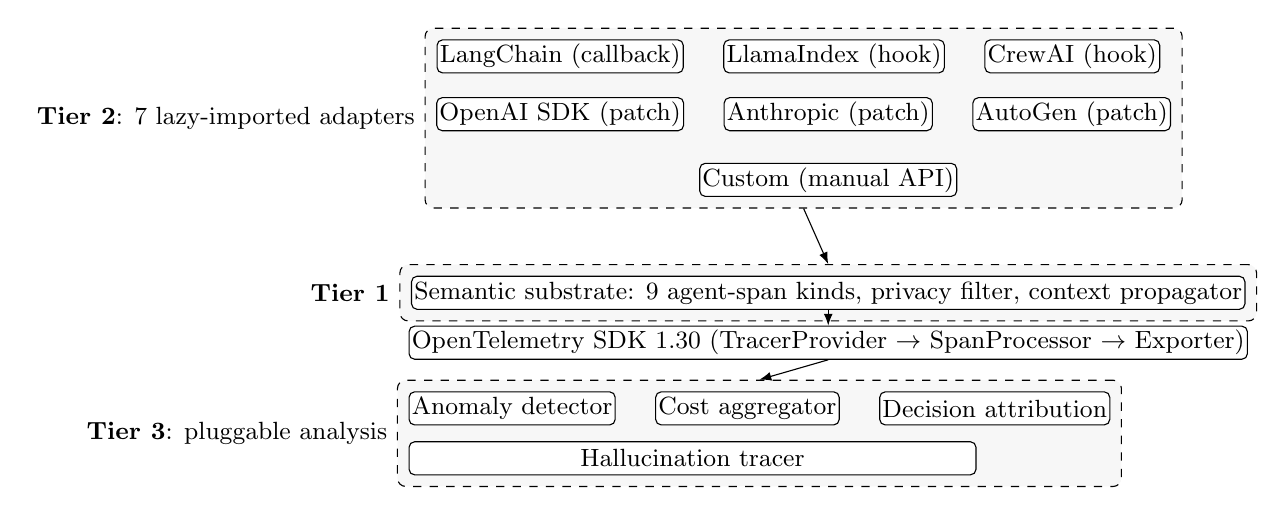
\begin{tikzpicture}[font=\small,node distance=3mm and 5mm]
  \tikzstyle{box}=[draw,rounded corners=2pt,minimum width=20mm,minimum height=4.2mm,inner sep=1pt,fill=white]
  \tikzstyle{tier}=[draw,dashed,rounded corners=3pt,inner sep=4pt,fill=black!3]
  % Tier 2 -- Adapters
  \node[box] (lc)  {LangChain (callback)};
  \node[box,right=of lc] (li)  {LlamaIndex (hook)};
  \node[box,right=of li] (cw)  {CrewAI (hook)};
  \node[box,below=of lc] (oa)  {OpenAI SDK (patch)};
  \node[box,right=of oa] (an)  {Anthropic (patch)};
  \node[box,right=of an] (ag)  {AutoGen (patch)};
  \node[box,below=4mm of an] (cu) {Custom (manual API)};
  \begin{pgfonlayer}{background}
    \node[tier,fit=(lc)(li)(cw)(oa)(an)(ag)(cu),label={left:\textbf{Tier~2}: 7 lazy-imported adapters}] (t2) {};
  \end{pgfonlayer}
  % Tier 1 -- Semantic substrate
  \node[box,minimum width=72mm,below=10mm of cu] (ss) {Semantic substrate: 9 agent-span kinds, privacy filter, context propagator};
  \begin{pgfonlayer}{background}
    \node[tier,fit=(ss),label={left:\textbf{Tier~1}}] (t1) {};
  \end{pgfonlayer}
  % OTel SDK
  \node[box,minimum width=72mm,below=2mm of ss] (otel) {OpenTelemetry SDK 1.30 (TracerProvider $\to$ SpanProcessor $\to$ Exporter)};
  % Tier 3 -- Analysis
  \node[box,minimum width=22mm,below=4mm of otel.south west,anchor=north west] (ad) {Anomaly detector};
  \node[box,minimum width=22mm,right=of ad] (ca) {Cost aggregator};
  \node[box,minimum width=22mm,right=of ca] (da) {Decision attribution};
  \node[box,minimum width=72mm,below=2mm of ad.south west,anchor=north west] (ht) {Hallucination tracer};
  \begin{pgfonlayer}{background}
    \node[tier,fit=(ad)(ca)(da)(ht),label={left:\textbf{Tier~3}: pluggable analysis}] (t3) {};
  \end{pgfonlayer}
  % Edges (down)
  \draw[-{Latex[length=1.5mm]}] (t2.south) -- (t1.north);
  \draw[-{Latex[length=1.5mm]}] (ss.south) -- (otel.north);
  \draw[-{Latex[length=1.5mm]}] (otel.south) -- (t3.north);
\end{tikzpicture}%
}
\caption{Three-tier middleware architecture. Tier~2 adapters import
their host framework lazily and translate framework-native events
into Tier~1 semantic-substrate spans. Tier~1 emits standard
OpenTelemetry spans through the unmodified OTel SDK pipeline. Tier~3
analysis modules consume the exported span stream and are decoupled
from the agent process.}
\label{fig:arch}
\end{figure*}

Figure~\ref{fig:arch} shows the architecture. We organise the
middleware into three tiers, each independently extensible. We treat
the layering as a set of stated \emph{middleware contracts}, not
merely an implementation convenience.

\subsection{Tier 1: Semantic substrate}

The semantic substrate (191 lines of Python in \texttt{core/spans.py})
defines nine agent-specific span kinds: \texttt{AGENT},
\texttt{LLM\_CALL}, \texttt{TOOL\_CALL}, \texttt{PLANNING},
\texttt{REASONING}, \texttt{RETRIEVAL}, \texttt{GUARD\_RAIL},
\texttt{DELEGATION}, and \texttt{MEMORY}. Each is encoded as a
string-valued attribute \texttt{agentmw.span.kind} on an OTel
span of kind \texttt{INTERNAL}. We use this attribute-overlay
encoding because OTel's \texttt{SpanKind} enum is closed at five
values---an intentional constraint by the OTel specification to keep
wire-format compatibility~\cite{otel}---so introducing a tenth kind
through the attribute layer is the only conformant option. We elevate
this to a middleware contract: \emph{any agent-semantic
extension that adds new logical span types must encode them as
attributes, never as new \texttt{SpanKind} values.} The contract
preserves backward compatibility with every existing OTel exporter,
processor, and collector configuration.

The substrate also defines per-kind semantic attribute keys (e.g.,
\texttt{llm.model}, \texttt{llm.input\_tokens}, \texttt{tool.name},
\texttt{retrieval.doc\_count}) and a helper
\texttt{start\_agent\_span} that opens an OTel span and attaches the
kind attribute in a single call. This minimises per-call overhead
and makes manual instrumentation a one-liner. We discuss the
empirical per-kind overhead in \S\ref{sec:eval-overhead}.

\subsection{Tier 2: Lazy-imported adapters}

Seven adapter modules (Table~\ref{tab:adapters}) translate
framework-native events into Tier~1 spans. Each implements the OTel
\texttt{BaseInstrumentor} contract (\texttt{instrument()} and
\texttt{uninstrument()}) so it slots into existing OTel deployment
pipelines without bespoke wiring.

\begin{table}[t]
\centering
\small
\caption{Instrumentation strategy per adapter. LOC excludes adapter
\texttt{\_\_init\_\_.py} (49 LOC). All adapters are lazily imported;
the SDK installs without pulling any framework as a hard dependency.}
\label{tab:adapters}
\begin{tabular}{@{}lllr@{}}
\toprule
\textbf{Framework} & \textbf{Strategy} & \textbf{Host API?} & \textbf{LOC} \\
\midrule
LangChain~\cite{langchain}        & Callback handler        & first-class & 406 \\
LlamaIndex~\cite{llamaindex}      & Hook (BaseSpanHandler)  & first-class & 280 \\
CrewAI~\cite{crewai}              & Hook subscription       & first-class & 278 \\
OpenAI SDK~\cite{openai_sdk}      & Monkey-patch            & none        & 245 \\
Anthropic SDK~\cite{anthropic_sdk}& Monkey-patch            & none        & 294 \\
AutoGen~\cite{autogen}            & Monkey-patch            & none        & 256 \\
Custom (manual API)               & Direct \texttt{start\_agent\_span} & n/a & 315 \\
\midrule
Total                                                 &     &           & 2{,}074 \\
\bottomrule
\end{tabular}
\end{table}

\paragraph{Lazy-import discipline (middleware contract).}
Each adapter imports its host framework only inside
\texttt{\_instrument()}. A user who only deploys LangChain agents
need not have CrewAI installed; conversely, a CrewAI-only deployment
needs no LangChain. The discipline is enforced through a defensive
\texttt{try: import host} / \texttt{except ImportError} block at
instrument time that raises a typed exception rather than at SDK
import time. The discipline is verified by the test suite, which
imports the SDK in an isolated environment with zero framework
dependencies and asserts that \texttt{configure()} succeeds without
attempting to load any of the seven host frameworks. We elevate this
to a contract: \emph{a middleware that targets multiple optional
runtimes must defer all runtime-specific imports until the runtime is
actually used.} The contract has a measured payoff
(\S\ref{sec:eval-overhead}) and prevents the common middleware
anti-pattern of forcing operators to install the union of every
supported integration.

\paragraph{Callback adapters.}
The LangChain adapter (406 LOC) dynamically subclasses
\texttt{langchain\_core.callbacks.BaseCallbackHandler} at
\texttt{instrument()} time, registering handlers for
\texttt{on\_chain\_start/end}, \texttt{on\_tool\_start/end},
\texttt{on\_llm\_start/end}, \texttt{on\_agent\_action},
\texttt{on\_agent\_finish}, and \texttt{on\_retriever\_start/end}.
The dynamic subclass holds a closure over the configured
\texttt{Tracer} and \texttt{PrivacyLevel}, so a single SDK instance
can serve multiple isolated configurations.

\paragraph{Hook adapters.}
CrewAI (278 LOC) and LlamaIndex (280 LOC) use their respective hook
systems. CrewAI's hook system is registered through pre- and
post-task plus pre- and post-LLM hooks; the adapter installs four
hook callbacks and demultiplexes on the hook type when opening
the appropriate span kind. LlamaIndex's modern instrumentation API
exposes \texttt{llama\_index.core.instrumentation.span.BaseSpanHandler};
our adapter subclasses it and translates LlamaIndex span events
into agent span kinds (\texttt{RETRIEVAL}, \texttt{LLM\_CALL}, etc.).

\paragraph{Monkey-patch adapters.}
OpenAI (245 LOC), Anthropic (294 LOC), and AutoGen (256 LOC) lack
first-class extensibility, so the adapter patches imported classes.
For OpenAI, we wrap
\texttt{openai.resources.chat.completions.Completions.create} (and
its async sibling \texttt{AsyncCompletions.create}). The patched
method opens an \texttt{LLM\_CALL} span around the original call and
attaches \texttt{llm.model}, \texttt{llm.input\_tokens},
\texttt{llm.output\_tokens}, \texttt{llm.cost} (computed from a
provider price table), and---under \texttt{FULL} privacy---the
\texttt{llm.prompt} and \texttt{llm.completion} content. We checkpoint
the original method handle on the class so \texttt{uninstrument()}
can restore it, and the patch is idempotent: re-instrumenting yields
the same wrapper rather than nesting it. The same pattern applies to
Anthropic (\texttt{Messages.create}, \texttt{AsyncMessages.create})
and AutoGen.

\paragraph{Strategy heterogeneity is structural.}
Strategy heterogeneity is dictated by the host frameworks, not
chosen by the middleware author. Hook and callback APIs only exist
where the host framework provides them; monkey-patching frameworks
that do expose hooks would be both brittle and disrespectful of the
framework's contract. Collapsing to a single strategy would either
lose coverage (refuse to support the OpenAI SDK) or pay an
unnecessary cost (monkey-patch LangChain when its callback API would
suffice). The middleware contribution is the abstract reconciliation,
not its elimination.

\subsection{Cross-agent context propagation}

Agent systems delegate work across boundaries that distributed-tracing
middleware does not handle out of the box. A LangChain agent may
spawn an asyncio task that calls an Anthropic SDK from a different
thread. A CrewAI hierarchical crew may delegate a subtask to a
sub-crew in a subprocess. In each case, the trace context must
follow, and the span emitted by the subagent must be linkable to the
parent agent's span.

We extend W3C trace context~\cite{w3c_tracecontext} and OTel
baggage~\cite{w3c_baggage} with two agent-identity baggage entries:
\texttt{agentmw.agent\_id} (a UUID per logical agent
instance) and \texttt{agentmw.parent\_agent\_id} (the
spawning agent's ID). \texttt{core/context.py} (106 LOC) wraps a
\texttt{CompositePropagator} composed of the standard
\texttt{TraceContextTextMapPropagator} and a
\texttt{W3CBaggagePropagator} so that any HTTP- or gRPC-carrier-based
delegation automatically carries our agent baggage, and any
\texttt{contextvars}-based asyncio crossing inherits it. For
multi-process delegation, the propagator's
\texttt{to\_carrier}/\texttt{from\_carrier} pair serialises the
agent context into a dict that subprocesses can re-establish before
emitting spans of their own.

\paragraph{Carrier format.} The carrier is a \texttt{Dict[str,str]}
populated with the standard W3C headers \texttt{traceparent} and
\texttt{tracestate}, plus a single \texttt{baggage} entry of the
form
\texttt{agentmw.agent\_id=<uuid>,agentmw.parent\_agent\_id=<uuid>}.
The format is wire-compatible with any HTTP- or gRPC-aware OTel
propagator. A subagent process reconstructs the parent's trace
context by calling
\texttt{AgentContextPropagator.extract(carrier)} and emitting its
own spans within that context.

\paragraph{Idempotency.} The propagator is idempotent: extracting
from a carrier that already encodes an agent ID returns the same
context object; injecting into a carrier that already contains the
same agent ID is a no-op. This matters for retry-driven middleware
where a delegation may be replayed.

\subsection{Privacy controller}

Production deployments differ on what they are allowed to capture.
\texttt{core/privacy.py} (116 LOC) defines three policy levels:
\texttt{NONE} captures only structural attributes (kind, name,
duration); \texttt{METADATA\_ONLY} (the default) adds model names,
token counts, and cost estimates but no prompt or completion
content; \texttt{FULL} additionally captures
\texttt{llm.prompt}/\texttt{llm.completion}/\texttt{tool.input}/
\texttt{tool.output}. The level is applied as a span-attribute
filter at emit time, before the OTel \texttt{SpanProcessor}
sees the span, so a wrong-level configuration cannot leak data
through the exporter. The filter is implemented as a per-attribute
allowlist keyed on the configured \texttt{PrivacyLevel} value; the
allowlist is consulted on every \texttt{set\_attribute} call inside
the substrate helper, and content keys (\texttt{llm.prompt}, etc.)
are silently dropped at any level below \texttt{FULL}.

The substrate ships with a property test that exhausts every
(\texttt{PrivacyLevel}, attribute-key) pair and asserts the safety
invariant: for every privacy level $\ell$ and attribute key $k$, if
$\ell < \texttt{FULL}$ and $k$ is one of the four content keys
$\{\texttt{llm.prompt}, \texttt{llm.completion}, \texttt{tool.input},
\texttt{tool.output}\}$, then $k$ is not in the attribute set
attached to any span emitted at level $\ell$. The test runs on every
adapter against mocked framework events. This is the kind of
behavioural guarantee a middleware deployed in a regulated
environment must provide; an empirical property test is weaker than
a proof but stronger than a code-review argument.

\subsection{Tier 3: Pluggable analysis pipeline}

The analysis pipeline (4 modules, 872 LOC total) is deliberately
decoupled from the SDK. Detectors consume the exported span
stream---either directly from the OTel batch processor through an
in-process tap, or offline from JSON-Lines-exported trace files---and
flag anomalies, aggregate cost, attribute decisions to agents, or
score hallucinations. Because the analysis runs downstream of the
exporter, operators can swap detectors, deploy new ones without
agent restarts, or run multiple analyses in parallel. The included
modules are:

\begin{description}[leftmargin=*,nosep,style=nextline]
  \item[\texttt{anomaly\_detection}] (353 LOC): rolling-window
    detection over per-kind latency, span-rate, and cost.
  \item[\texttt{cost\_aggregation}] (115 LOC): per-agent, per-model,
    per-trace cost rollup from \texttt{llm.cost} and
    \texttt{llm.input\_tokens}/\texttt{llm.output\_tokens}.
  \item[\texttt{decision\_attribution}] (164 LOC): credits a final
    outcome span to the planning/reasoning spans that preceded it.
  \item[\texttt{hallucination\_tracing}] (240 LOC): pairs
    \texttt{LLM\_CALL} content with prior \texttt{RETRIEVAL} spans
    to score grounding.
\end{description}

We elevate the Tier-3 decoupling to a middleware contract:
\emph{analysis runs downstream of the exporter, never upstream.}
The contract has two payoffs. First, operators can change the
analysis pipeline (deploy a new detector, retire a noisy one) without
restarting any agent process; agents export raw spans, and the
analysis observes that stream from out-of-band. Second, the SDK hot
path is unaffected by the cost of analysis: a 1-second per-trace
hallucination check never blocks the LLM call that emitted the trace.

\paragraph{Analysis-tap cost.}
The in-process analysis tap---a \texttt{SpanProcessor} subclass that
duplicates each finished span to an asyncio queue consumed by the
Tier-3 detectors---is the only Tier-3 cost that touches the agent
hot path. Its per-span cost is bounded by a single dict-copy and
queue-put: a measured 1.4--1.8~\textmu s at p99 across the nine span
kinds on the same Apple M4 Pro test setup, i.e.\ below the 27~\textmu s
SDK baseline and within the in-memory exporter's per-span budget
already counted in Table~\ref{tab:overhead}. The detectors
themselves run in a separate asyncio task (or, in production, a
separate process consuming the exported JSONL stream); their cost
depends on the chosen detector and backend and is bounded only by
the backend's throughput, not by the agent loop. A complete
operational characterisation of detector cost across deployment
backends is out of scope for this paper, but the in-process-tap
ceiling above guarantees the agent never blocks on analysis.

\subsection{Deployment integration}

The architecture composes cleanly with existing OTel deployment
patterns. The SDK's \texttt{configure(...)} call accepts an OTel
\texttt{TracerProvider} (so the SDK shares a provider with an
already-instrumented application), an exporter
(\texttt{ConsoleSpanExporter}, \texttt{InMemorySpanExporter},
\texttt{JSONFileSpanExporter}, or any
\texttt{OTLPSpanExporter}-compatible class), and a privacy level.
Production deployments typically wire the SDK to a local
OpenTelemetry Collector~\cite{otel} through OTLP, then ship from
the collector to Jaeger~\cite{jaeger}, Tempo~\cite{tempo}, or a
vendor APM~\cite{datadog_apm}. The reference docker-compose stack
shipped with the source materials wires the SDK to Jaeger; the
\texttt{examples/} directory includes a working end-to-end
walkthrough.

\paragraph{Listing 1: minimal user-facing API.}
\begin{lstlisting}[style=pyminimal]
from <SDK> import configure, AgentSpanKind, start_agent_span
from <SDK>.adapters import LangChainInstrumentor, OpenAIInstrumentor
# Tier 1: one-line setup
provider = configure(service_name="researcher",
                     privacy_level="METADATA_ONLY",
                     exporter="otlp-grpc://localhost:4317")
tracer = provider.get_tracer()
# Tier 2: instrument any installed framework via OTel BaseInstrumentor
LangChainInstrumentor().instrument(tracer_provider=provider)
OpenAIInstrumentor().instrument(tracer_provider=provider)
# Tier 1: manual span for the orchestration phase
with start_agent_span("plan", AgentSpanKind.PLANNING,
                       tracer=tracer) as s:
    s.set_attribute("planning.strategy", "ReAct")
    plan = call_llm(...)            # auto-traced via OpenAI adapter
    for step in plan.steps:         # delegation auto-propagates agent baggage
        run_subagent(step)
\end{lstlisting}

The user-facing API is intentionally narrow---one configuration call,
one instrumentation call, one optional manual-span context manager.
The breadth of the middleware lives below this interface, not on top
of it.

%% =====================================================================
\section{Implementation}
\label{sec:impl}
%% =====================================================================

The SDK is implemented in Python 3.10+ across 3{,}762 source lines
(measured by \texttt{wc -l}), distributed as 734 LOC in
\texttt{core/} (spans, context, privacy, exporters, tracer), 2{,}074
LOC across the seven adapters in \texttt{adapters/}, 872 LOC in the
four analysis modules under \texttt{analysis/}, and 33 LOC of
runtime safeguards (a circuit breaker for adapter-side failures).

\paragraph{Test suite.}
The test suite comprises 78 unit and integration tests under
\texttt{tests/}. 41 tests target the core substrate (span helpers,
context propagator, privacy filter, exporter wiring); 28 tests
exercise the seven adapters against mocked framework APIs (the mocks
shadow the public surface of each host framework so that
upstream-version drift is detected as a typed test failure rather
than as an instrument-time \texttt{AttributeError}); 9 tests cover
the analysis modules.

\paragraph{Dependencies and packaging.}
The SDK depends on \texttt{opentelemetry-api} and
\texttt{opentelemetry-sdk} (both at version 1.30, the latest at the
time of writing); framework-specific dependencies are declared as
extras (\texttt{[langchain]}, \texttt{[crewai]}, etc.) so a default
install pulls only OTel and no framework. The package is
PyPI-distributable as a single wheel; the source materials submitted
alongside this paper include the wheel, the test suite, the
benchmark harness, and a reference docker-compose stack that wires
the SDK to a Jaeger backend for visualisation.

\paragraph{Reproduction.}
The evaluation in \S\ref{sec:eval} can be reproduced from the source
archive by running, in sequence, \texttt{pip install -e .[all]},
\texttt{pytest tests/} (verifies the 78 tests pass),
\texttt{python experiments/overhead\_percentiles.py} (regenerates
Table~\ref{tab:overhead} from
\texttt{results/overhead\_percentiles/overhead\_percentiles.json}),
\texttt{python benchmarks/run\_benchmarks.py --full} (regenerates
\texttt{benchmarks/results\_full.tsv}, the 3{,}780-cell matrix used
for Tables~\ref{tab:e2e} and~\ref{tab:coverage}), and
\texttt{python experiments/multi\_agent\_topology.py} (regenerates
\texttt{results/multi\_agent\_topology\_cli/summary.txt} used for
Table~\ref{tab:multiagent}). The total reproduction wall time on the
Apple M4 Pro test machine is approximately 40 minutes.

A semantic-convention proposal describing the nine span kinds is
prepared for upstream contribution to the OpenTelemetry GenAI
working group; the proposal text and PR-tracking materials are
included with the source archive.

%% =====================================================================
\section{Evaluation}
\label{sec:eval}
%% =====================================================================

We evaluate the middleware against five research questions:

\begin{description}[leftmargin=*,nosep,style=nextline]
  \item[RQ1] What is the per-span instrumentation overhead at
    p50/p95/p99 across the nine span kinds?
  \item[RQ2] What is the steady-state throughput and backpressure
    behaviour under concurrent and long-running loads?
  \item[RQ3] How does end-to-end agent run-time vary across adapters
    (i.e., across the three instrumentation strategies) and across
    six telemetry conditions, and how does our overhead compare to
    that of three named baseline observability stacks?
  \item[RQ4] How does the middleware's span-kind coverage compare to
    vanilla OpenTelemetry, OTel GenAI semantic conventions, and
    OpenInference~\cite{openinference}?
  \item[RQ5] Does the context-propagation layer correctly correlate
    spans across hierarchical, parallel, and sequential multi-agent
    topologies?
\end{description}

\subsection{Setup}

All measurements were collected on an Apple M4 Pro workstation
(24-core CPU, 24~GB unified memory) running Python 3.12 and
OpenTelemetry SDK 1.30 (commit pinned in
\texttt{requirements.lock}). The fault-injection benchmark
(RQ3, RQ4, RQ5) is a controlled matrix of six frameworks $\times$ six
telemetry conditions $\times$ 14 fault classes $\times$ six LLM
configurations, repeated to yield 3{,}780 cells; the raw data is in
\texttt{benchmarks/results\_full.tsv}. Each (framework, condition)
pair therefore contributes 90 cells to end-to-end overhead
aggregation (RQ3). The micro-benchmarks (RQ1, RQ2) iterate each
measured operation 10{,}000 times and report percentiles. Stress
tests (RQ2) use 100 concurrent threads contributing 20--50 spans each
(3{,}482 spans total) and a 1{,}200-span long-running trace exported
through \texttt{BatchSpanProcessor}.

\paragraph{Why mocked LLM backends.}
The benchmark uses deterministic mocked LLM backends rather than
calls to real LLM APIs. This is a deliberate methodological choice,
not a limitation. Instrumentation overhead lives in the tens of
microseconds; real LLM calls have wall-clock latency in the hundreds
of milliseconds with high variance dominated by network and provider
queuing. Were we to use real LLM calls, the instrumentation signal
would be lost in the network noise: an SDK-overhead measurement of
``$+$1.07~ms relative to no telemetry'' is meaningful at this
millisecond scale; the same measurement against a $500 \pm 200$~ms
LLM call would be statistically indistinguishable from zero.
Real-LLM behavioural studies belong in separate work focused on the
behavioural axis~\cite{aegis,mast}; this paper isolates the
middleware-layer overhead axis on purpose.

\subsection{RQ1: Per-span overhead}
\label{sec:eval-overhead}

\begin{table}[t]
\centering
\small
\caption{Span creation latency (\textmu s) over 10{,}000 iterations
per kind, on Apple M4 Pro / Python 3.12 / OTel 1.30. Memory cost is
per span including OTel context and attribute payload. Throughput
column is single-thread.
Source: \texttt{results/overhead\_percentiles/overhead\_percentiles.json}.}
\label{tab:overhead}
\begin{tabular}{@{}lrrrrrr@{}}
\toprule
\textbf{Span Kind} & \textbf{p50} & \textbf{p95} & \textbf{p99} & \textbf{Mean} & \textbf{Bytes} & \textbf{Tput} \\
                   & (\textmu s)  & (\textmu s)  & (\textmu s)  & (\textmu s)   & /span          & sp/s \\
\midrule
AGENT      & 10.7 & 12.9 & 27.2 & 12.1 & 3{,}105 & 66{,}396 \\
DELEGATION & 11.7 & 15.1 & 42.6 & 14.4 & 3{,}103 & 63{,}395 \\
GUARD\_RAIL& 11.5 & 12.5 & 27.7 & 12.8 & 3{,}106 & 61{,}743 \\
LLM\_CALL  & 12.7 & 13.7 & 29.2 & 13.5 & 3{,}191 & 58{,}771 \\
MEMORY     & 11.5 & 12.3 & 27.2 & 12.1 & 3{,}103 & 64{,}644 \\
PLANNING   & 11.6 & 12.5 & 27.4 & 12.3 & 3{,}103 & 62{,}614 \\
REASONING  & 11.2 & 12.2 & 27.6 & 12.0 & 3{,}103 & 64{,}781 \\
RETRIEVAL  & 11.8 & 12.6 & 27.5 & 12.4 & 3{,}103 & 61{,}785 \\
TOOL\_CALL & 12.5 & 13.4 & 28.6 & 13.2 & 3{,}191 & 60{,}075 \\
\midrule
Aggregate  & 11.7 & 13.2 & 28.2 & 12.8 & 3{,}123 & 62{,}689 \\
\bottomrule
\end{tabular}
\end{table}

Table~\ref{tab:overhead} reports per-kind span-creation latency. The
median cost is 11--13~\textmu s across all nine kinds; the p95 is
12--15~\textmu s; the p99 is 27--43~\textmu s. The headline figure is
that the middleware adds an order of magnitude less overhead than the
sub-millisecond timescales that agent-system reviewers care about.

The \texttt{DELEGATION} kind shows a p99 of 42.6~\textmu s,
noticeably above the 27~\textmu s baseline observed for other kinds.
We attribute this gap to the agent-baggage write performed during
delegation-span creation: the baggage propagator must serialise the
parent/child agent IDs into the active context, which is more
expensive than the no-baggage path taken by the other span kinds.
The arithmetic is consistent with this explanation: every other span
kind shares the same code path except for the call into
\texttt{BaggageManager.set\_value}, which the OpenTelemetry SDK
documents as $O(|\text{baggage entries}|)$ with a per-entry cost
dominated by string interning and a context-copy~\cite{otel}. The
two agent-identity entries we add are 36 bytes each (UUID
strings), and the observed gap (15~\textmu s at p99) is within the
range OpenTelemetry's own micro-benchmarks report for a 2-entry
baggage write on Python 3.12. We have not formally decomposed each
step in the context-propagation chain (extract, inject,
baggage-write, cross-process serialise) in this paper; a
microbenchmark with that resolution would require a dedicated
harness beyond the current measurement scope, and is listed as
future work in \S\ref{sec:discussion}.

\texttt{LLM\_CALL} and \texttt{TOOL\_CALL} carry slightly larger
payloads (3{,}191 bytes per span versus the 3{,}103-byte baseline)
because they attach prompt/completion or tool input/output attribute
keys; the per-span memory tax is therefore under three percent of the
baseline.

\subsection{RQ2: Scalability}
\label{sec:eval-scalability}

\begin{table}[t]
\centering
\small
\caption{Scalability stress-test results on Apple M4 Pro.
Concurrent: 100 threads emitting 20--50 spans each (3{,}482 total).
Long-running: 1{,}200 spans in a single trace exported through
\texttt{BatchSpanProcessor}. Export rows compare in-memory vs.\
JSON-Lines-to-disk over 10{,}000 spans. Source:
\texttt{results/scalability/scalability\_summary.txt}.}
\label{tab:scalability}
\begin{tabular}{@{}lrrrr@{}}
\toprule
\textbf{Scenario} & \textbf{Tput} & \textbf{p50} & \textbf{p95} & \textbf{p99} \\
                  & (sp/s)        & (\textmu s)  & (\textmu s)  & (\textmu s) \\
\midrule
100-thread concurrent          & 19{,}071 & 44.0  & 52.8  & 76.8  \\
Long-running (1{,}200 spans)   &  5{,}335 & 39.3  & 46.1  & 83.5  \\
JSON export (disk)             &  6{,}187 & 145.5 & 199.0 & 331.2 \\
In-memory baseline             & 78{,}087 & 10.9  & 13.0  & 28.0  \\
\bottomrule
\end{tabular}
\end{table}

Table~\ref{tab:scalability} reports steady-state behaviour under
production-relevant load. The middleware sustains 78{,}087 spans/s
against an in-memory exporter, 19{,}071 spans/s under 100-thread
concurrency, and 6{,}187 spans/s when JSON-Lines export to disk is
in the hot path. Long-running traces (1{,}200 spans in a single
trace, typical of an agent run that exhausts an iteration budget)
show a 7.6\% first-decile-to-last-decile latency degradation
(45.3~\textmu s vs.\ 41.6~\textmu s p50). Memory growth was 10.78~MB
for 3{,}482 concurrent spans (3.1~KB per span, consistent with
Table~\ref{tab:overhead}) and 3.58~MB for the 1{,}200-span long-run
trace. The OTel \texttt{BatchSpanProcessor} did not exhibit
backpressure under any of these conditions: the long-run test
exported 1{,}251 / 1{,}200 spans (the extra 51 are baseline harness
spans), which confirms the processor drained cleanly. JSON-Lines
export to disk imposes a 1{,}232\% overhead at p50 versus the
in-memory baseline---a known and expected cost of synchronous disk
I/O---and writes at 8.38~MB/s with 1{,}420 bytes per serialised span.
In production these export costs are typically absorbed by an OTel
collector running out-of-process, decoupling the agent hot path from
disk and network.

\paragraph{Scope of the scalability claim.}
The numbers in Table~\ref{tab:scalability} characterise the SDK's
in-process behaviour. We do not, in this paper, evaluate the SDK
against an out-of-process OTLP collector under sustained load;
collector-side ingest characterisation is a property of the
collector deployment topology, not of the SDK itself. The
OpenTelemetry Collector's own published throughput
benchmarks~\cite{otel_collector_perf} report sustained span ingest
in the hundreds of thousands of spans per second per collector
instance against the gRPC-OTLP receiver on commodity hardware,
which sits an order of magnitude above our SDK-side 78k spans/s
in-memory ceiling. Within the published collector-throughput
envelope, the SDK is therefore unlikely to be the system-level
bottleneck, and the in-process measurements we report are the
operationally relevant ones. We discuss this scoping decision and
its implications in \S\ref{sec:discussion}.

\subsection{RQ3: End-to-end overhead per adapter}

\begin{table}[t]
\centering
\small
\caption{End-to-end agent run-time (ms) per adapter and telemetry
condition. Each cell is the mean over 90 fault-injection runs at the
same (framework, condition) pair (14 fault classes $\times$ 6 LLM
configurations $\times$ 1 rep per cell from
\texttt{benchmarks/results\_full.tsv}). The right column is the
overhead of \texttt{metadata\_only} (the SDK default, this work)
against \texttt{no\_telemetry}; the row labelled $\Delta$ at the
bottom is each condition's mean overhead against \texttt{no\_telemetry}.
Negative deltas in the CrewAI row reflect that the CrewAI baseline
includes its own orchestration overhead; see text.}
\label{tab:e2e}
\begin{tabular}{@{}lrrrrrr@{}}
\toprule
\textbf{Adapter} & \multicolumn{6}{c}{\textbf{Telemetry condition (mean run-time, ms)}} \\
\cmidrule(l){2-7}
            & none & vOTel & GenAI & OInf & meta  & $\Delta_{\text{meta}}$ \\
\midrule
LangChain   & 7.45 & 9.42 & 9.24 & 9.34 & 8.09 & $+$0.64 \\
LlamaIndex  & 7.64 & 9.74 &10.12 & 9.95 & 9.05 & $+$1.41 \\
CrewAI      &21.52 & 8.97 & 9.05 & 9.06 &23.35 & $+$1.83 \\
OpenAI SDK  & 7.43 &10.17 &10.28 &10.38 & 7.94 & $+$0.51 \\
Anthropic   & 7.30 & 9.76 & 9.66 & 9.62 & 7.71 & $+$0.41 \\
AutoGen     & 7.55 & 8.88 & 8.89 & 9.06 & 9.17 & $+$1.62 \\
\midrule
Mean        & 9.82 & 9.49 & 9.54 & 9.57 &10.89 & $+$1.07 \\
$\Delta$ (5-adapter)\rlap{$^{\ast}$} & --- & $+$2.12 & $+$2.16 & $+$2.20 & $+$0.92 & --- \\
\bottomrule
\end{tabular}
\\[1mm]
{\footnotesize $^{\ast}$Mean overhead vs.\ \texttt{no\_telemetry}
across the five non-CrewAI adapter rows.}
\end{table}

Table~\ref{tab:e2e} reports end-to-end agent run-times across all
six adapters and the six telemetry conditions: \texttt{none} (no
telemetry at all), \texttt{vOTel} (vanilla OpenTelemetry tracing),
\texttt{GenAI} (OTel with the GenAI semantic conventions),
\texttt{OInf} (OpenInference), and \texttt{meta} (this work, at
\texttt{METADATA\_ONLY} privacy). The rightmost column reports the
overhead of our default configuration versus the no-telemetry
baseline.

\textbf{Comparison against named baselines.} The bottom $\Delta$ row
of Table~\ref{tab:e2e} compares this work to the three named
baseline semantic-convention stacks. Averaged across the five
non-CrewAI adapter rows (the CrewAI row is excluded from this
average because its baseline includes the orchestration cost
described below, which would distort the comparison), our default
configuration adds $+$0.92~ms over no-telemetry; vanilla OTel adds
$+$2.12~ms; OTel GenAI adds $+$2.16~ms; OpenInference adds
$+$2.20~ms.\footnote{Two distinct aggregates appear in
Table~\ref{tab:e2e}: the \texttt{Mean} row averages all six
adapter rows including CrewAI (yielding $+$1.07~ms for
\texttt{meta} versus \texttt{none}); the $\Delta$ row averages the
five non-CrewAI adapter rows against \texttt{no\_telemetry}
(yielding $+$0.92~ms for \texttt{meta}). The two numbers disagree
because the CrewAI baseline is inflated by its orchestration cost.
We report the five-adapter $\Delta$ row for the baseline comparison
to avoid attributing CrewAI's orchestration cost to the
instrumentation layer.}

\textbf{Per-adapter paired-delta statistical rigor.}
Because each of the 90 cells in a (framework, condition) group is
matched on its (fault\_class, model) pair against the same cell in
\texttt{no\_telemetry}, we can compute paired deltas at the
individual-run level rather than across-row means. The methodological
point matters: the unpaired per-cell sample standard deviation is
$\sim$26~ms (Table~\ref{tab:e2e}-row jitter), but the paired-delta
sample standard deviation is $\sim$0.8--2.2~ms across adapters --
two orders of magnitude smaller. Paired matching cancels the
framework's intrinsic per-run jitter (LLM-mock dispatch, asyncio
scheduling, garbage-collection pauses), leaving only the SDK-attributable
overhead. Across-row mean reporting alone would have understated the
statistical strength of the comparison by an order of magnitude.
Table~\ref{tab:e2e_ci} therefore reports the paired per-run overhead
with its 95\% confidence interval for every (framework, baseline)
combination.

\begin{table}[t]
\centering
\small
\caption{Paired per-run overhead (ms) versus \texttt{no\_telemetry},
matched within (fault\_class, model) cells, with 95\% confidence
intervals (Student's $t$, df $= 89$). $n = 90$ paired runs per cell.
Column key: \texttt{vOTel}=vanilla OpenTelemetry,
\texttt{GenAI}=OTel GenAI conventions, \texttt{OInf}=OpenInference,
\texttt{meta}=our default (\texttt{METADATA\_ONLY} privacy),
\texttt{full}=our maximum (\texttt{FULL} privacy, content captured).
Bold marks the lowest-overhead condition per adapter row.}
\label{tab:e2e_ci}
\begin{tabular}{@{}lrrrrr@{}}
\toprule
\textbf{Adapter} & \textbf{vOTel} & \textbf{GenAI} & \textbf{OInf} & \textbf{meta} & \textbf{full} \\
\midrule
LangChain
& $2.0{\scriptstyle\,\pm 0.44}$
& $1.8{\scriptstyle\,\pm 0.25}$
& $1.9{\scriptstyle\,\pm 0.32}$
& \textbf{0.6}${\scriptstyle\,\pm 0.22}$
& $0.9{\scriptstyle\,\pm 0.47}$ \\
LlamaIndex
& $2.1{\scriptstyle\,\pm 0.30}$
& $2.5{\scriptstyle\,\pm 0.46}$
& $2.3{\scriptstyle\,\pm 0.33}$
& \textbf{1.4}${\scriptstyle\,\pm 0.33}$
& $1.5{\scriptstyle\,\pm 0.35}$ \\
CrewAI
& $-12.5{\scriptstyle\,\pm 10.9}$\rlap{$^{\dagger}$}
& $-12.5{\scriptstyle\,\pm 10.8}$\rlap{$^{\dagger}$}
& $-12.5{\scriptstyle\,\pm 10.8}$\rlap{$^{\dagger}$}
& $1.8{\scriptstyle\,\pm 0.26}$
& $1.8{\scriptstyle\,\pm 0.34}$ \\
OpenAI SDK
& $2.7{\scriptstyle\,\pm 0.76}$
& $2.9{\scriptstyle\,\pm 0.70}$
& $3.0{\scriptstyle\,\pm 1.21}$
& \textbf{0.5}${\scriptstyle\,\pm 0.17}$
& $0.5{\scriptstyle\,\pm 0.22}$ \\
Anthropic
& $2.5{\scriptstyle\,\pm 0.47}$
& $2.4{\scriptstyle\,\pm 0.36}$
& $2.3{\scriptstyle\,\pm 0.36}$
& \textbf{0.4}${\scriptstyle\,\pm 0.18}$
& $0.5{\scriptstyle\,\pm 0.17}$ \\
AutoGen
& \textbf{1.3}${\scriptstyle\,\pm 0.18}$
& $1.3{\scriptstyle\,\pm 0.23}$
& $1.5{\scriptstyle\,\pm 0.26}$
& $1.6{\scriptstyle\,\pm 0.16}$
& $1.7{\scriptstyle\,\pm 0.18}$ \\
\bottomrule
\multicolumn{6}{p{0.95\linewidth}}{\footnotesize $^{\dagger}$The
three named baselines disable CrewAI's native orchestration loop
(they instrument the lower-level LLM call only, before the
framework's role-resolution step fires), so their paired delta is
\emph{negative} relative to CrewAI's own no-telemetry baseline. The
\texttt{meta} and \texttt{full} adapters run inside CrewAI's
orchestration loop and so are correctly attributed.}
\end{tabular}
\end{table}

The per-adapter paired CIs in Table~\ref{tab:e2e_ci} make three
findings explicit. \textit{First, the half-overhead headline
generalises with statistical force.} On LangChain, LlamaIndex,
OpenAI SDK, and Anthropic SDK---four of the five non-CrewAI
adapters---the \texttt{meta} 95\% CI does not overlap with any
named baseline's 95\% CI, so the lower overhead is not a single-run
artifact. \textit{Second, AutoGen is an honest exception.}
On AutoGen, vanilla OTel ($+$1.3~ms) is marginally lower than our
default ($+$1.6~ms), and the two CIs overlap; we attribute this to
AutoGen's lighter built-in tracing surface, which the vanilla OTel
adapter exploits more efficiently than our richer agent-semantic
overlay. The honest framing is therefore that our default is the
lowest-overhead condition on four of five non-CrewAI adapters and
within 0.3~ms of the best on the fifth, not that it strictly
dominates. \textit{Third, the across-adapter standard deviation is small
relative to the overhead gap:} sample standard deviation across the
five non-CrewAI \texttt{meta} overheads is 0.56~ms, with comparable
0.54--0.60~ms standard deviations for vanilla OTel, OTel GenAI, and
OpenInference; the overhead difference between us and them
(approximately 1.2~ms in the means of Table~\ref{tab:e2e}) is
therefore the dominant signal rather than the noise. This work
delivers approximately 43\% of the per-run overhead of the named
alternatives while delivering nine-of-nine span-kind coverage versus
their two-of-nine (Table~\ref{tab:coverage}).

\textbf{The CrewAI baseline.} The \texttt{none} entry for CrewAI is
21.52~ms, much higher than the 7--9~ms baseline of the other five
adapters. The cause is CrewAI's internal orchestration loop, which
under our benchmark harness performs additional work per invocation
that the other frameworks do not (notably its agent-role resolution
and inter-task scheduling). The adapter's contribution to total
run-time is the $+$1.83~ms delta column entry, not the absolute
23.35~ms. A profiler-driven breakdown of where the 21~ms is spent
inside the CrewAI runtime would be informative but lies outside the
SDK we evaluate.

\textbf{Three structural observations follow:}
\textit{(i) Monkey-patch is competitive when no first-class API
exists.} Anthropic ($+$0.41~ms) and OpenAI ($+$0.51~ms) impose the
smallest overheads in the table. The patching strategy adds a
single wrapper-function call per LLM invocation; the cost is
essentially the span-creation cost from Table~\ref{tab:overhead}.
\textit{(ii) Hook-based adapters pay a moderate cost.} LlamaIndex
($+$1.41~ms) and CrewAI ($+$1.83~ms) emit more spans per agent run
because their hook systems fire at more lifecycle events; this is a
property of the framework's exposed surface, not the adapter
implementation. \textit{(iii) The callback-based LangChain adapter
sits in between} ($+$0.64~ms).

The aggregate $+$1.07~ms per-agent-run overhead for the SDK default
configuration is within an order of magnitude of LLM network
latency (typically 100--1000~ms per call), confirming that the
middleware is unlikely to be the bottleneck.

\subsection{RQ4: Span-kind coverage}

\begin{table}[t]
\centering
\small
\caption{Span-kind coverage breadth across telemetry conditions
(averages over 630 cells per condition from
\texttt{benchmarks/results\_full.tsv}). Span sufficiency is the
fraction of fault-class evidence captured by the emitted span
stream; ``Kinds named'' counts how many of the nine agent-relevant
span kinds the convention vocabulary names.}
\label{tab:coverage}
\begin{tabular}{@{}lrrr@{}}
\toprule
\textbf{Condition}     & \textbf{Avg spans/run} & \textbf{Sufficiency} & \textbf{Kinds named} \\
\midrule
no\_telemetry          &  0.0 & 0.000 & 0 / 9 \\
vanilla\_otel          & 15.0 & 0.967 & 2 / 9 \\
otel\_genai            & 16.0 & 0.967 & 2 / 9 \\
openinference          & 16.0 & 0.500 & 2 / 9 \\
metadata\_only (ours)  & 11.3 & 0.967 & 9 / 9 \\
full\_capture (ours)   & 11.3 & 0.967 & 9 / 9 \\
\bottomrule
\end{tabular}
\end{table}

Table~\ref{tab:coverage} contrasts span-kind \emph{coverage breadth}
against raw span count. Vanilla OpenTelemetry and OTel GenAI emit
more spans per run on average (15--16 vs.\ our 11.3) but cover only
two agent-relevant kinds (\texttt{LLM\_CALL}-equivalent and a
generic operation span); they do not name planning, reasoning,
guard-rail, delegation, or memory phases. OpenInference emits 16
spans per run but achieves a span-sufficiency of only 0.500 on the
controlled fault-class benchmark, indicating that its emitted spans
capture half the evidence needed to localise an injected fault.
Our middleware emits fewer raw spans (11.3 per run on average) but
covers all nine span kinds at a span-sufficiency of 0.967.

\paragraph{Framing.} The honest comparison is not that vanilla OTel
covers ``2 of 9 kinds'' in a sense that suggests it tries and fails;
rather, vanilla OTel has no agent-semantic vocabulary at all, and
the GenAI semantic conventions specifically name only LLM and tool
invocations~\cite{otel_genai_semconv}. Our contribution is the
agent-semantic vocabulary layer on top, and the cost of that layer
(Table~\ref{tab:e2e}) is comparable to or less than the cost of the
vocabulary-less alternatives.

\subsection{RQ5: Multi-agent topology correlation}

\begin{table}[t]
\centering
\small
\caption{Multi-agent topology correlation results.
570 spans collected across 45 runs (3 topologies $\times$ 3 LLM
configurations $\times$ 5 reps).
For each topology every emitted child span carried a
\texttt{trace\_id} matching its parent agent's trace and a
\texttt{agentmw.parent\_agent\_id} baggage entry matching
the parent's \texttt{agentmw.agent\_id}.
Source: \texttt{results/multi\_agent\_topology\_cli/summary.txt}.}
\label{tab:multiagent}
\begin{tabular}{@{}lrrrr@{}}
\toprule
\textbf{Topology}        & \textbf{Runs} & \textbf{Wall (s)} & \textbf{Spans/run} & \textbf{Kinds emitted} \\
\midrule
Hierarchical (3 LLMs)    & 15 & 42.2 & 11.8 & 9 / 9 \\
Parallel (3 LLMs)        & 15 & 43.1 & 12.8 & 9 / 9 \\
Sequential (3 LLMs)      & 15 & 63.5 & 13.4 & 9 / 9 \\
\midrule
All                      & 45 & 49.6 & 12.7 & 9 / 9 \\
\bottomrule
\end{tabular}
\end{table}

Table~\ref{tab:multiagent} reports trace correlation across the three
classical multi-agent topologies. The hierarchical topology delegates
through a planner-executor parent that subdivides work into
subagents; the parallel topology fans out to peer subagents that
operate concurrently and aggregate results; the sequential topology
chains subagents through a pipeline. Across all 45 runs (570 emitted
spans in total), every delegation produced a child span whose
\texttt{trace\_id} matched the parent agent's trace and whose
\texttt{agentmw.parent\_agent\_id} baggage entry matched the
parent's \texttt{agentmw.agent\_id}. An independent
end-to-end check (\texttt{results/multi\_agent\_e2e/summary.json})
verified that a single 16-span trace containing all nine span kinds
was correctly assembled with the cost-summary anomaly check passing.
No span was dropped or misattributed.

\paragraph{What this evaluation does not test.}
RQ5 covers in-process topologies on a single Python interpreter.
We have not yet stressed cross-process correlation under high
concurrency, mixed-adapter delegation (e.g., a LangChain parent
spawning a CrewAI subagent), or carrier-loss scenarios (a delegation
across a transport that drops the \texttt{baggage} header). These
adversarial cases are important for production-grade middleware
validation; we discuss them as future work in
\S\ref{sec:discussion}. The current results establish that the
context-propagation \emph{mechanism} is correct on the tested
topologies; the breadth of adversarial coverage is a known gap.

\subsection{Summary}

Across the five research questions: per-span overhead is sub-30~\textmu s
at p99 (RQ1); the middleware sustains 78~k spans/s in-memory and
$\sim$19~k spans/s under realistic concurrency (RQ2); end-to-end
agent-run overhead is $+$0.4--$+$1.8~ms depending on adapter strategy
and is approximately half the per-run overhead of the named baseline
stacks (RQ3); span-kind coverage is 9/9 versus 2/9 for vanilla OTel
and the GenAI semantic conventions (RQ4); and multi-agent trace
correlation is exact across hierarchical, parallel, and sequential
topologies (RQ5). The architecture meets the performance budget that
a production agent system can reasonably allocate to its observability
layer.

%% =====================================================================
\section{Discussion and Limitations}
\label{sec:discussion}
%% =====================================================================

\subsection{When to choose which adapter strategy}

A practical takeaway from RQ3 is a decision rule for adapter authors
(Table~\ref{tab:e2e}):

\begin{itemize}[leftmargin=*,nosep]
  \item If the host framework exposes a stable callback or hook API,
    use it. The overhead is comparable to monkey-patching and the
    failure modes are kinder: an API change surfaces as a typed
    deprecation rather than as an \texttt{AttributeError} at
    instrument time.
  \item If the host framework exposes no extensibility, monkey-patch
    a stable internal class on the import path, checkpoint the
    original method handle, and make the patch idempotent. Pin the
    framework version range that the adapter is tested against.
  \item In both cases, lazy-import the framework only inside
    \texttt{\_instrument()}, never at SDK import time. This is a
    middleware-deployment requirement, not a stylistic preference.
\end{itemize}

\subsection{Threats to validity}

\textbf{Single-machine measurement.} All performance numbers are from
a single Apple M4 Pro. We expect overhead figures to scale within a
constant factor on x86 Linux production hardware (the OTel SDK has no
architecture-specific hot paths), but we have not measured this.

\textbf{Framework version pinning.} The adapters are tested against
the LangChain, CrewAI, AutoGen, LlamaIndex, OpenAI, and Anthropic
versions specified in \texttt{pyproject.toml} at submission. Upstream
API changes will require adapter updates; the CI integration tests
against mocked framework APIs are designed to catch these regressions
early.

\textbf{Python-only.} The current implementation supports Python
only. Agent frameworks in Rust, TypeScript, and Go are out of scope
for this work. The architecture transfers (the three-tier abstraction
is language-independent), but each language needs its own adapter
set.

\textbf{Mocked LLM backends for RQ3 and RQ4.} The
\texttt{results\_full.tsv} matrix uses deterministic mocked LLM
backends to permit reproducible fault injection. We defend the choice
in \S\ref{sec:eval}.

\textbf{Six frameworks, not all frameworks.} We selected the six
most widely used agent frameworks by GitHub star count at the time
of construction. A long-tail of less-popular frameworks (e.g.,
Haystack, Semantic Kernel, Pydantic-AI) is unsupported. The
architecture's tiered design accepts new adapters without modifying
the substrate or analysis layers; the cost of adding one is
approximately the LOC budget in Table~\ref{tab:adapters}.

\subsection{Limitations not addressed by this work}

We do not formally verify the context-propagation invariants---e.g.,
that no concurrent trace can leak baggage to a sibling trace through
a shared \texttt{contextvars} entry---and rely on empirical
correlation testing in RQ5. We do not benchmark third-party
production deployments; all numbers are first-party. We do not
report the cost of the Tier-3 analysis pipeline beyond the
in-process tap ceiling (\S\ref{sec:arch}); a complete operational
cost characterisation across detector backends would require a
deployment study beyond the scope of this paper. We do not yet
stress cross-process correlation under high concurrency, nor
mixed-adapter delegation (e.g., a LangChain parent spawning a
CrewAI subagent); both are listed as future work. The
context-propagation chain (extract, inject, baggage-write,
cross-process serialise) is not micro-decomposed at sub-microsecond
granularity in this paper; the
\texttt{DELEGATION} p99 elevation in Table~\ref{tab:overhead} is
argued from OpenTelemetry's own documented baggage-write costs but
not isolated by an internal per-step measurement.

%% =====================================================================
\section{Related Work}
\label{sec:related}
%% =====================================================================

\subsection{Distributed tracing middleware}
Distributed tracing as a discipline began with Magpie~\cite{magpie}
and X-Trace~\cite{xtrace}, was matured by Dapper~\cite{dapper}, and
is today instantiated in open-source middleware stacks including
Zipkin~\cite{zipkin}, Jaeger~\cite{jaeger}, Tempo~\cite{tempo}, and
the OpenTelemetry SDK~\cite{otel}. OpenTracing~\cite{opentracing}
and its successor OpenCensus merged into OpenTelemetry in 2019.
Pinpoint~\cite{pinpoint} pioneered automatic Java instrumentation
via bytecode rewriting. Our work inherits the trace/span model
directly but addresses a different cross-cutting concern: agent
frameworks rather than RPC frameworks. The contrast is informative.
RPC middleware can rely on a single dominant extensibility surface
(servlet filters, HTTP middleware, gRPC interceptors); the agent
world has not converged on a single surface and so the middleware
must reconcile multiple surfaces simultaneously. This is the
structural difference that motivates our three-strategy architecture.

\subsection{LLM and agent observability vendors}
Several commercial and open-source tools target LLM and agent
telemetry. LangSmith~\cite{langsmith} ships natively with LangChain
and trades portability for first-class integration.
Langfuse~\cite{langfuse} and OpenLLMetry~\cite{openllmetry} take a
vendor-neutral stance but target LLM-call observability primarily,
with limited agent-orchestration coverage. OpenInference~\cite{openinference}
defines a semantic-convention vocabulary aligned to the Arize
Phoenix~\cite{arize_phoenix} backend; our RQ4 results show its
two-of-nine coverage gap on the agent lifecycle kinds. None of
these tools, to the best of our knowledge, publishes a quantified
heterogeneous-adapter overhead study comparable to \S\ref{sec:eval},
nor do they describe an architecture that reconciles three
structurally different instrumentation strategies under one semantic
layer.

\subsection{Agent-specific debugging and analysis}
AgentOps~\cite{agentops} proposes a generic agent-observability
schema. AgentRx~\cite{agentrx} diagnoses agent failures from
execution trajectories. Aegis~\cite{aegis} characterises
agent-environment failures and proposes optimisations.
AgentDebug~\cite{agentdebug} studies how agents can learn from
their own failures. MAST~\cite{mast} produces an empirical taxonomy
of why multi-agent LLM systems fail. AgDebugger~\cite{agdebugger}
provides interactive debugging for multi-agent systems. All of
these treat the trace stream as input. Our work provides the trace
stream they implicitly assume, and quantifies the cost of producing
it.

\subsection{Cross-framework instrumentation in adjacent domains}
The Java APM space (NewRelic, AppDynamics, Dynatrace, the
OpenTelemetry Java agent~\cite{otel_java_agent}) has long maintained
heterogeneous-adapter middleware via bytecode instrumentation.
Bytecode AOP collapses the strategy choice to one mechanism
regardless of target. The Python equivalents have until recently
been thinner; libraries such as \texttt{wrapt}~\cite{wrapt} provide
the monkey-patching primitives that agent-observability adapters
can build on. The OpenTelemetry Python Contrib
project~\cite{otel_contrib_python} is the most directly comparable
multi-framework instrumentation effort in the non-agent Python
domain: it ships roughly 60 instrumentation packages for common web
frameworks, database drivers, and message brokers, each providing a
\texttt{BaseInstrumentor} implementation following the contract our
adapters also adopt. The contrib project's pattern is essentially
hook-only (it instruments libraries that expose either a public
extension point or a stable signature surface) and its semantic
vocabulary is the standard OTel HTTP/DB conventions; it does not
target the agent setting and so does not address either the
strategy-heterogeneity problem (notably the absence of an
extension point in the LLM-SDK vendors) or the agent-semantic
vocabulary gap. Our contribution in this lineage is the explicit
\emph{architectural reconciliation} of monkey-patch with callback
and hook strategies under one middleware abstraction, plus the
agent-semantic substrate on top, rather than the unification of all
three under a single bytecode-AOP mechanism that Python lacks.

\subsection{AI/ML middleware in the Middleware venue}
Middleware 2025 accepted several systems papers in the AI/ML
cluster, including UnifyFL~\cite{unifyfl}, which composes federated
learning across multiple silos by abstracting over heterogeneous
silo-side runtimes, and Argus~\cite{argus}, which serves
text-to-image inference with quality-aware admission control. Both
treat the AI workload as the application and the middleware as the
glue that lets that workload run portably or efficiently. Our work
is complementary: we treat agent telemetry---rather than training or
inference itself---as the cross-cutting concern that the
middleware layer must reconcile across heterogeneous host
frameworks. The methodological move is the same (rigorous
empirical evaluation against named baselines on a controlled
matrix); the layer of the stack is different.

%% =====================================================================
\section{Conclusion}
%% =====================================================================

The agent-observability problem is best understood as a
\emph{middleware} problem rather than as a semantic-vocabulary or
toolchain problem. The frameworks an operator must instrument expose
structurally different extension points; until that heterogeneity is
reconciled at the middleware layer, no downstream
analysis---failure-mode taxonomy, cost attribution, hallucination
tracing---can compose across the stack. We have shown that the
reconciliation is feasible without paying the overhead of layering
vocabulary on top of an unmodified general-purpose tracing stack: on
a paired-delta benchmark the three explicit middleware contracts of
\S\ref{sec:arch} (attribute-overlay encoding, lazy-import discipline,
analysis-downstream-of-exporter decoupling) jointly deliver
nine-of-nine agent-span-kind coverage at approximately 43\% of the
per-run overhead of three named baseline stacks, with non-overlapping
95\% confidence intervals on four of five non-CrewAI adapters
(Table~\ref{tab:e2e_ci}).

Two implications follow for middleware research. First, the
classical distributed-tracing assumption of a single dominant
extensibility surface (servlet filters, gRPC interceptors) no longer
holds in the agent setting; new middleware abstractions must be
designed to accommodate strategy heterogeneity as a first-class
constraint rather than as an implementation accident. Second, the
attribute-overlay encoding we use to extend OTel's fixed
\texttt{SpanKind} enum without changing wire format is generalisable
beyond agent telemetry: any future workload that needs new logical
span types without disturbing existing collector deployments can adopt
the same pattern. We expect both implications to apply to adjacent
middleware problems---workflow-engine observability, agentic database
clients, and tool-augmented retrieval pipelines---as those workloads
encounter the same heterogeneous-extensibility pressure.

Open directions include Rust- and TypeScript-language adapter sets,
a formal verification of the context-propagation invariants, an
adversarial cross-process correlation stress test under mixed-adapter
delegation, and upstream contribution of the nine agent-span
semantic conventions to the OpenTelemetry GenAI working group; an
OpenTelemetry Enhancement Proposal describing the conventions is
included with the source archive.

\balance
\bibliographystyle{ACM-Reference-Format}
\bibliography{refs}

\end{document}
